\chapter[Tools and technology used]{Tools and technology used}

This thesis's outcome can not be achived without the tools and technologies
used to develop, debug and test. With the right tools, we can make the work
easier and faster. In this chapter we list the tools and technologies used to
make our desire forensics tool.

\section[The C++ language]{The C++ language}

C++ is an old language, first developed by Bjarne Stroustrup in 1985 as a
complement to the C language. C++ delivers better type checking and more
\textit{notational support}. With its strong compatibility with C and its
strictness, C++ is a better programming language for enterprise-level projects.

The transition from C to C++ is slowly adapted to OS programming. The Windows
operating system supports writing drivers using C++. However, using C++ in the
kernel is very difficult. In the kernel space, there is no runtime. In other
words, no standard library, no exception handling, no constructor for global
objects.  Although most C++ features are still available: classes, range-for
loop, lambda, templating.

Writing the kernel driver in C++ will make the code easier to manage and
extend. That is why we are using C++ when developing the kernel driver.

\section[The Rust language]{The Rust language}

Rust is a new language developed by Graydon Hoare. It first appears in 2010.
The language is designed to eliminate the bad design in concurrent programming
languages while retaining the program's efficiency and speed.  Regardless of
its age, many successful projects have been made with Rust. Rust makes the code
safety from compile-time to runtime by checking for memory access during
compilation. Rust captures attention from system programmer, from Microsoft to
Linux developers, all are considering using Rust in their future projects and
planning to use Rust with the system.

We use Rust to develop the user application. Rust can interface C structures
and call native Windows API easily. With the speed comparable to C++ and the
safety that Rust gives, choosing Rust was a brilliant idea.

\section[WinDbg]{WinDbg}

WinDbg is a debugger, a tool used to debug other programs, made by Microsoft.
WinDbg was first developed for the developer to inspect the crash dump produced
when the Windows crash. However, it can later be used to debug a running
machine through a wire connection. WinDbg fetches the debug symbols
automatically and use it to help developers debug the problem. In 2017,
Microsoft announced a remake of WinDbg, WinDbg Preview, with stunning graphics
and new features.

\section[VirtualBox]{VirtualBox}

We are developing a tool used inside the kernel space. It is advised to use an
isolated environment for testing. By using a hypervisor, a software that
simulates the hardware to run an OS, we get an isolated environment.
VirtualBox is a hypervisor distributed under Oracle and is free to use.
VirtualBox can run a wide range of Windows versions, which is suitable for
testing multiple Windows versions. VirtualBox can be set up to debug the
running operating system with WinDbg, as in Figure \ref{fig:windbg}.

\begin{figure}[h]
  \centering
  \caption{WinDbg debugging Windows 7 on VirtualBox}
  \label{fig:windbg}
  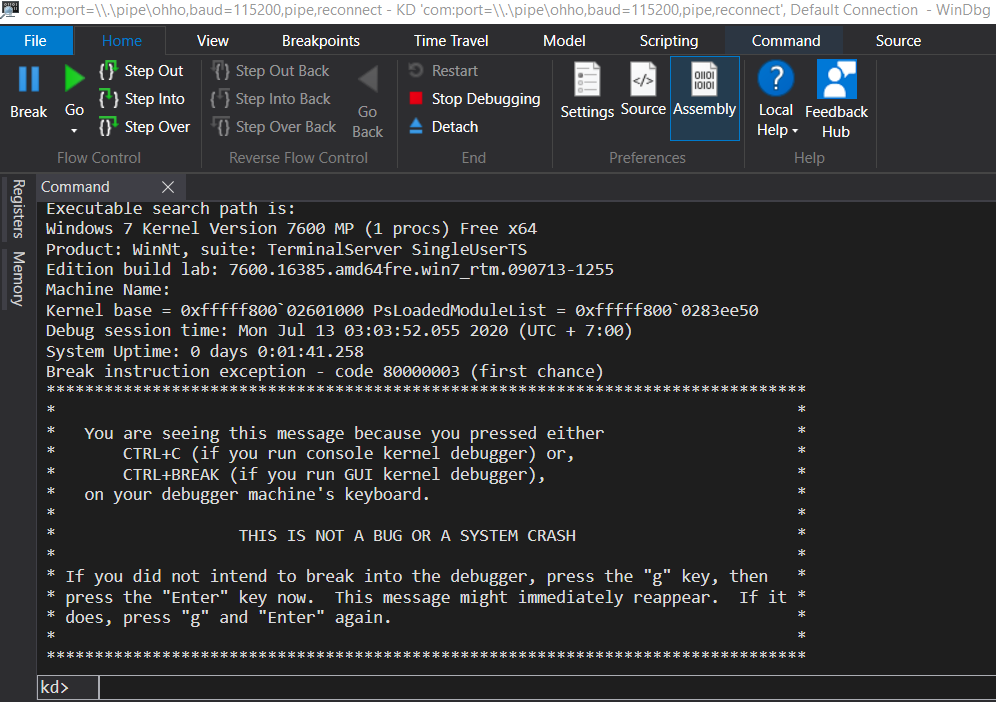
\includegraphics[scale=0.4]{images/windbg.png}
\end{figure}
